\documentclass[a4paper,12pt]{report}
\usepackage[top=2.5cm, bottom=2.5cm, left=2.5cm, right=2.5cm]{geometry}
\usepackage[utf8x]{inputenc}
\usepackage[T1]{fontenc}
\usepackage[french]{babel} 
\usepackage{graphicx}
\usepackage{hyperref}
\usepackage{url}
\makeatletter
\g@addto@macro{\UrlBreaks}{\UrlOrds}
\makeatother

\author{\textsc{Jorandon} Guillaume, \textsc{Marcoux} Vincent\\\small{Responsable pédagogique : \textsc{Collomb} Cléo}}
\date{22 mai 2017} 
\title{
\includegraphics[width=140px]{utc.jpg}\\\vspace{25mm}Discriminations et algorithmes\\\normalsize{SC22 P17}}

\begin{document}

\hypersetup{pageanchor=false}
\maketitle
\tableofcontents
\hypersetup{pageanchor=true}
\chapter*{Introduction}
\addcontentsline{toc}{chapter}{Introduction}
Nous vivons aujourd'hui dans un monde où l'évolution technologique est très rapide, et où on ne peut plus ne pas avoir entendu parler des algorithmes, nouveaux outils techniques omniprésents. Dans la société qu'est la notre, hyper-technologique, il est en effet difficile de les éviter, et ils nous apparaissent comme des outils très utiles et faciles à utiliser. Ces algorithmes sont pour partie le fait de grands groupes qui recherchent le profit, et qui dans cet objectif exploitent des corrélations statistiques pour générer de l'information exploitable. En faisant passer un grand volume de données connectées au travers d'algorithmes toujours plus efficaces, ces acteurs industriels majeurs peuvent faire du profilage sur la population : c'est ce qu'on appelle la fouille de données, enseignée à l'UTC dans la filière FDD du Génie Informatique, et que l'on rassemble parfois sous le terme vague de \textit{Big Data}. Ce savoir constitue un ``pouvoir statistique'' énorme qui confère aux entreprises qui le possèdent une force de frappe politique et économique considérable, et est source d'une certaine forme de gouvernance, la gouvernementalité algorithmique. Comme toute source de pouvoir, il convient alors de la questionner et de se demander dans quel mesure elle est légitime. Peut-elle être discriminatoire, subjective, guidée par une certaine idéologie, ou est-elle neutre et objective ? Sur qui ou quoi faire reposer la responsabilité des dérives de cette gouvernementalité algorithmique ? Mais surtout, peut-on parler de discrimination algorithmique ? 

Dans le cadre de l'UV SC22, nous avons travaillé sur une approche culturelle des techniques, notamment au travers des prismes de genre et de classe. Dans ce cadre, nous avons étudié l'origine de certains mécanismes systémiques, sources d'oppressions et de discriminations : sexistes, raciales, sur l'identité sexuelle et de genre, etc. En nous appuyant sur le cours mais aussi sur l'étude de plusieurs articles, nous allons essayer de définir ce qu'est la gouvernementalité algorithmique et son fonctionnement. Nous verrons dans quelles mesures les discriminations algorithmiques s'inscrivent dans cette gouvernementalité. Nous étudierons plusieurs exemples pour illustrer nos propos.

\chapter{Gouvernementalité Algorithmique}

Nous devons d'abord commencer par définir clairement la notion de gouvernementalité algorithmique, avant même de pouvoir essayer d'en étudier les effets. C'est l'objet de ce premier chapitre, qui repose en partie sur \cite{nps}.

\section{Qu'est-ce que la gouvernementalité algorithmique ?}

Tout d'abord, commençons par définir ce que sont les gouvernements. Il faut prendre l'activité de gouvernement au sens large : les éducateur/ices, les directeur/ices, les parents, les professionnel-le-s du marketing, etc. Il ne faut donc pas considérer que c'est l'État qui détient le monopole de l'activité gouvernementale. L'évolution de l'informatique et des éléments technologiques qui l'entourent permet l'enregistrement massif des données, ce qui génère une révolution du pouvoir et engendre une sorte de numérisation de la vie sans être ``a priori'', une menace pour les droits individuels, le respect de la vie privée et des données personnelles. En effet, les individus eux-mêmes y contribuent en laissant spontanément, volontairement ou non des traces numériques. S'appuyant sur une série de dispositifs technologiques de détection, de classification, d'évaluation prédictive, anticipative (parfois autonome) des comportements humains, la puissance de ce gouvernement réside dans des algorithmes, des corrélations statistiques, donc la gouvernementalité algorithmique.

L'objectif d'un gouvernement privé ou public est d'anticiper les actions possibles des individus, de prévoir le futur d'un actuel à peine discernable, par exemple prévoir les intentions de consommation, les intentions criminelles... ``Diriger c'est prévoir''. La gouvernementalité algorithmique semble émerger, lorsque la quantité d'éléments à analyser est trop grande (multitude de citoyen-ne-s, diversité culturelle, nationalités diverses...). Elle procure les avantages de confort, d'efficacité tant du gouvernement public et privé, qu'aux individus eux-mêmes et donc au travers de dispositifs de biométrie dynamique, de vidéosurveillance et d'environnement intelligent, d'informatique omniprésente fonctionnant de manière autonome (on approche l'intelligence artificielle). Elle ne rencontre que très peu de récalcitrance parce que se basant sur un ``réel'', elle gouverne le potentiel de champ d'action d'individus auxquels elle ne s'adresse que de manière indirecte.

\section{De la gouvernementalité algorithmique au pouvoir statistique}

Nous allons voir les différentes étapes qu'utilise la gouvernementalité algorithmique pour pouvoir générer son savoir statistique, et donc son pouvoir.

La numérisation des comportements humains individuels ou collectifs, n'est plus limitée en capacité d'une part vu l'évolution ``technico-économique'', d'autre part par un refus des individus parce que la collecte des données est généralisée et anonyme et que la suppression de celle-ci nécessite de la part de l'individu une démarche active et souvent compliquée.
Cette digitalisation crée une masse de données permettant une qualité de prédiction indépendante du caractère sophistiqué des algorithmes.

Le \textit{data mining} indifférent au pourquoi (causalité) des phénomènes est l'application de la technologie et des techniques de banques de données (comme l'analyse statistique et la modélisation) dans le but de découvrir les structures cachées et les relations subtiles entre données, et d'en induire des règles (normes) permettant la prédiction de résultats futurs en fouillant dans la quantité très grande de données brutes disponibles, sorte de ``mémoire digitale totale''. Les objectifs du \textit{data mining} sont l'amélioration des prestations et des services, la détection d'activités criminelles (ex: le terrorisme), des fraudes, des gaspillages et abus, l'analyse d'informations scientifiques et de recherche (diagnostic médical...), la gestion des ressources humaines...
A partir de ce \textit{data mining} on peut établir le profilage algorithmique. Vu la diversité anarchique des comportements humains, le profilage algorithmique permet de déduire (à partir de corrélation sur de nombreuses données) des caractéristiques individuelles non observables, actuelles ou futures à partir de la seule présence de certaines caractéristiques observables chez un individu (ex : profil de consommateur/ices, de risques...).

Les profils ne visent personne en particulier, ils ne s'intéressent pas aux individus en tant qu'individus (c'est la dividualisation des personnes), ils assignent les mêmes prédictions comportementales à tous ceux qui se trouvent présenter un certain nombre d'éléments repris dans lesdits profils quelques soient leurs caractères propres \footnote{Par exemple, un-e étudiant-e quelqu'il soit achète très certainement des pâtes.}. Le profilage tend à s'universaliser, en évinçant la relation de causalité.

Le gouvernement utilise le \textit{data mining} et le profilage pour pouvoir faire des prédictions et de la préemption des comportements des individus (tout en gérant les incertitudes affiliées), par exemple la prévention du terrorisme, risque économique, et financier.

\section{L'individu dans la gouvernementalité algorithmique}

Nous allons voir maintenant la considération de l'individu par la gouvernementalité algorithmique. 

Le pouvoir s'intéresse à cet ``être'' numérique, issu de données multiples, dynamiques et hétérogènes, images d'existences individuelles dont il ignore la spécificité, la subjectivité (qui se rapporte à un sujet).
L'individu unique et rationnel devient un ``dividu'' sans conscience, constitué de parties indépendantes, dispersées à la fois infra-personnelles (les données) et supra-personnelles (les profils). L'individu en tant que tel n'est plus subjectivé (reconnu) et devient un fournisseur de données et générateur de profil.
Le pouvoir d'un régime de gouvernementalité statistique n'attend plus du sujet qu'il soit unifié, assujetti aux normes, mais il tolère les incohérences des individus dont il produit le corps statistique en fonction de ce que ce corps pourrait faire. Il transforme les sujets moraux en simples coordonnées dans des tables statistiques de calculs (actuariels) et gouverne en se passant de toute relation réflexive de l'individu à la norme morale ou à la règle du droit, bannissant la notion d'obéissance ou de désobéissance à la loi et les catégories juridiques du dommage de celle-ci.

Grâce à cette considération et à la dividualisation des personnes, la gouvernementalité algorithmique se protège quoi qu'elle puisse faire paraître, dire ou même sous entendre et ne peut être l'atteinte juridiquement. Car en effet, vu que les méthodes de profilage dynamique classent les individus dans une multitude de catégories hétérogènes, sans différenciation ethnique, politique, religieuse..., la contestation collective à ce pouvoir devient impensable. Le réel touché par ce gouvernement n'est plus composé que de corps statistiques, par opposition au ``corps vivant'' corps physique, susceptible d'événements.

Par ailleurs, sa force vient de la possibilité qu'elle a de gouverner les comportements des sujets comme si ces comportements appelaient un tel gouvernement. Ces objectifs à la fois descriptifs et normatifs, reposant sur un réel composé par les sujets eux-mêmes et les traces qu'ils laissent font que la puissance de ce type de gouvernement apparaît comme inoffensive.

La gouvernementalité algorithmique va bien plus loin dans sa considération du pouvoir (par les individus), elle arrive non seulement à le faire paraître inoffensif mais aussi admiré par les individus. Ils adhèrent entièrement à leur propre gouvernementalité statistique par la répétition des traces qu'ils laissent sans instance extérieure de surveillance active. On peut se poser alors la question sur les intentions, les intérêts de ce gouvernement.

Contrairement au modèle de la société disciplinaire, où le pouvoir s'exerce sur des individus identifiés, assujettis par la norme, respectant les institutions et contrôlés selon leur fonction (par exemple, le gendarme ne commet pas d'infraction en public), le gouvernement algorithmique ignore les corps individuels (unités) et les populations (masses). Il s'exerce par la prédiction et la préemption des comportements basées sur le \textit{data mining}, le profilage algorithmique et la structuration du champ d'action possible des individus.

Lorsque l'individu est mécontent du gouvernement algorithmique, il y aurait comme moyen légal la juridiction mais celle-ci connaît des défaillances, des défauts face au pouvoir statistique. En effet, les régimes juridiques (et la norme qu'ils représentent) attachés à l'individu, au sujet de droit sont totalement inaptes à fournir aux individus les moyens de réagir, de résister, d'obtenir un droit à l'anonymat, face à la digitalisation de la vie même de la gouvernementalité statistique ou algorithmique.

Selon de nombreuses études, les régimes juridiques de protection de la vie privée et de la protection des données personnelles sont difficiles à appliquer, voir inadéquats face au recueil massif et continu de données personnelles, de leur traitement et de leur conservation (par défaut) à des fins inconnues que réalise la gouvernementalité algorithmique. De plus, le caractère personnel de ces données est difficilement attestable puisque ce gouvernement ne s'intéresse qu'aux fragments ``dividuels'' de celles-ci. Cependant, celui-ci a la possibilité d'agir sur l'environnement des individus, par exemple,malgré l'anonymat garanti des données, on peut identifier les sujets concernés par corrélations de celles-ci.

\section{Droit et consentement}

On peut donc en conclure sur cette partie que la gouvernementalité algorithmique de corrélations statistiques nous contrôle sur notre comportement actuel et futur. Elle oriente à notre insu et avec notre ``consentement'' nos choix de tous types, par exemple : commerciaux/ales, professionnel-le-s voire criminel-le-s, et de ce fait est omniprésente dans notre vie.

Façonnée par les événements du ``réel'', elle crée en permanence de nouvelle normes ; en effet, les éléments enregistrés peuvent enrichir, modifier et rendre les normes immanentes aux corps statistique. On peut dire à ce sujet que contrairement à la statistique classique qui vérifie une hypothèse, la statique algorithmique produit des hypothèses.

Le pouvoir et le gouvernement nous paraissent inoffensifs puisque qu'ils sont pratiquement indiscernables. Cependant, la suppression de plusieurs droits comme le droit à l'anonymat, à la désobéissance, à s'exprimer et comparaître (d'un point de vue juridique) rend cette gouvernementalité contraignante. Il faudrait de ce fait changer les normes juridiques quant au respect de la vie privée et des données personnelles. De plus, les algorithmes sont probabilistes ; on peut donc se poser la question sur leurs exactitudes (les corrélations sont-elles valables ? ). Sous cet éclairage, elle peut introduire une discrimination algorithmique malgré la dividualisation ``des données et de leur application `` ( \textit{data mining} et profilage).

\chapter{Discrimination algorithmique}

Nous venons donc de définir ce que sont le pouvoir et la gouvernementalité algorithmique, ainsi que leur influence sur la société comprenant les individus. Nous avons fini cette explication par la possibilité de cette gouvernementalité à être discriminatoire. Il est important pour la suite de définir ce qu'est la discrimination et comment nous l'entendons pour répondre à la problématique principale qui est ``existe- t'il des discriminations algorithmiques''.
Nous commencerons par la définir puis nous traiterons plusieurs exemples.

\section{Qu'est-ce que la discrimination ?}

Le mot discrimination vient du latin \textit{discriminis} qui signifie ``séparation''. Le sens du terme est à l'origine neutre, synonyme du mot distinction, mais il a pris, dès lors qu'il concerne une question sociale, une connotation péjorative désignant l'action de créer une disctinction de façon arbitraire, comme le fait de séparer un individu ou un groupe social des autres en le traitant de manière moins favorable dans une situation comparable.
La discrimination peut se rapporter à de nombreux facteurs, notamment on parle de discriminations :

\begin{itemize}
 \item sexuée (liée au genre supposé ou réel de la personne) ; 
 \item sexuelle (liée à l'orientation sexuelle) ;
 \item raciale et ethnique (liée à la couleur de peau, à l'origine supposée ou réelle) ;
 \item religieuse (liée à l'appartenance supposée ou réelle à une religion) ;
 \item sociale (liée à la classe sociale, au métier, à la condition) ;
 \item etc.
\end{itemize}

La discrimination peut être directe ou indirecte. Les cas de discrimination directe sont ceux où la discrimination est évidente dans les faits. Par exemple, le refus d'embaucher une personne parce qu'elle est d'origine nord-africaine, quel que soit le facteur qui permet de supposer de son origine (couleur de peau, accent, consonance du patronyme, etc.), est une discrimination directe. De même, refuser l'accès d'un lieu à une personne handicapée sous prétexte qu'elle est en chaise roulante est une autre forme de discrimination directe.

La discrimination indirecte en revanche est moins apparente à première vue. Ce genre de discrimination est bien plus répandu que la discrimination directe. Par exemple, une politique exigeant que les candidats à un emploi possèdent un permis de conduire semble neutre, et pourtant elle exclut les candidats qui ne peuvent obtenir un permis de conduire en raison par exemple d'un trouble mental ou neurologique (épilepsie par exemple).

\section{Le mythe de l'algorithme objectif}

Il est largement admis que les logiciels et algorithmes qui reposent sur une très grande quantité de données brutes, infra-dividuelles, sont objectifs. 

\begin{quotation}
A la différence des méthodes plus anciennes de profilage catégoriel, le profilage plus dynamique et individualisé que permettent les techniques de datamining classent les individus dans une multitude de catégories hétérogènes les unes aux autres, d'une très grande plasticité, constamment évolutives, de telle manière que, ces classifications ne recoupant aucune catégorisation socialement éprouvée (appartenance ethnique, genre, préférences sexuelles, opinions politiques, convictions religieuses…), leur contestation aux moyens d'actions collectives devient impensable, quels que soient de fait leurs effets potentiellement discriminatoires (Antoinette \textsc{Rouvroy}).
\end{quotation}

On peut expliquer ce potentiel discriminant par le fait que les algorithmes sont écrits par leurs concepteurs et entretenus par les utilisateurs. Les algorithmes d'auto apprentissage (\textit{machine learning} : où les ordinateurs apprennent par essais et erreurs à affirmer eux-mêmes leurs profils) ajustent ce qu'ils font en fonction du comportement des gens. Ces algorithmes peuvent renforcer les préjugés humains. De plus, les corrélations statistiques sont-elles fiables ?

Non, les algorithmes ne sont pas neutres, eux aussi peuvent discriminer. En effet, ce sont bel et bien des cerveaux humains qui élaborent les algorithmes, et qui déterminent avant cela à quels problèmes ils devront répondre. Ainsi, selon Süddeutsche  \textsc{Zeitung} : \begin{quote} Le racisme et le sexisme sont omniprésents dans les résultats des algorithmes automatisés et ce n'est pas parce que les ordinateurs ne sont pas neutres, mais parce qu'ils se basent sur ce que les grands groupes de gens pensent.\end{quote}

\textit{The Wall Street Journal} publiait qu'un noir-américain avait découvert\footnote{\url{https://blogs.wsj.com/digits/2015/07/01/google-mistakenly-tags-black-people-as-gorillas-showing-limits-of-algorithms/}} que l'algorithme de reconnaissance de Google avait classé une photo d'une amie noire comme étant celle d'un ``gorille''.
Une recherche de l'Université de Harvard en 2013 a également montré que lorsque l'on cherche des noms à consonnance africaine dans un moteur de recherche, celui-ci affiche plus fréquemment des dossiers d'arrestation. Aux États-Unis, des chercheurs de l'Université de Washington ont constaté qu'en tapant CEO, le moteur de recherche affichait uniquement des photos d'hommes blancs alors que près d'un tiers de PDG américains sont des femmes.

\section{Plusieurs exemples pour comprendre}

\subsection{Uber et Ubérisation}

On peut aussi citer les discriminations racistes et sexistes des plateformes de service telles que Uber et Airbnb. Notamment, l'application smartphone Uber permet de louer un VTC très facilement. Elle met en relation des passagers et chauffeurs grâce à un principe basé sur le \textit{big data}, le \textit{crowdsourcing}\footnote{La production participative, plus connue sous la dénomination anglaise \textit{crowdsourcing} consiste à regrouper les besoins ou souhaits de personnes compétentes pour résoudre des problèmes, puis de diffuser de manière libre la réponse à tout individu. Elle utilise la créativité, l'intelligence et le savoir-faire collectif pour mettre en commun les connaissances. C' est relatif à de la gestion de connaissances par le biais d'un travail collaboratif qui peut être réalisé soit par des spécialistes, soit par le grand public. Le \textit{crowdsourcing} est plus utilisé dans le monde du travail. Il permet à l'entreprise de développer une idée, un projet à l'aide d'internautes et cela contre rémunération. Seul problème : les internautes peuvent se sentir lésé-e-s du fait du décalage entre l'aide apportée (idée et solution) et la rémunération perçue. Il y a une injustice dans ce fonctionnement, on peut y reconnaître une forme de gouvernementalité (car c'est l'entreprise ici qui est décisionnelle) qui tire profit des individus alors qu'ils consentent à donner de l'information. Cette injustice peut se traduire par une ``discrimination de reconnaissance''. Cela vient du fait que ``tout travail mérite salaire'', l'internaute n'étant pas payé-e proportionnellement au gain perçu par la partie gouvernementale, iel se sent lésé-e et non reconnu à sa juste valeur. Il est à noter aussi que sur un appel à projet de \textit{crowdsourcing}, seul-e(s) lae ou les internaute(s) sélectionné-e(s) par l'entreprise seront rémunéré-e(s). L'injustice se situe alors pour celles et ceux qui auront consacré leur temps et leur réflexion pour rien ; on retrouve beaucoup ce problème dans le monde de la création graphique, où les artistes ont du mal à faire valoir leur métier.}.

Quiconque est disposé-e à proposer ses services de conducteur peut, au travers de l'application, gagner sa vie. Durant chaque trajet, Uber collecte et analyse des données pour déterminer la demande selon les zones géographiques. L'entreprise analyse également les réseaux de transport public de façon à se concentrer sur les zones non desservies. elle a développé des algorithmes pour surveiller les conditions de trafic et les temps de trajet en temps réel. Ainsi, les prix sont ajustés à mesure que la demande et les temps de trajet fluctuent : c'est le \textit{surge pricing}, introduisant une discrimination par les prix.

Une étude réalisée par les chercheurs du MIT a démontré qu'à Boston comme à Seattle, les demandes provenant des personnes dont le nom a une consonance renvoyant à une supposée couleur de peau noire sont deux fois plus annulées que les autres. Uber a réagi en ne révélant le nom du client que quand le chauffeur accepte la course. En retour, le temps d'attente s'allonge : il est deux fois plus long pour les personnes non blanches.
Dernier constat observé par l'étude, sexiste cette fois : lorsque le client est une femme, les bavardages du chauffeur se multiplient, les courses s'allongent et les clientes peuvent être aménées à être exposées à des ``coûts de voyage supplémentaires''.

On peut également mentionner le management par algorithme pratiqué par Uber et la précarisation des travailleurs. Le recours massif à des auto-entrepreneur/euses permet de diminuer les coûts tout en permettant aux travailleur/euses d'avoir un contact direct avec leurs client-e-s et d'être libres de décider de leurs horaires. Cependant, iels n'ont aucune marge de manoeuvre dans la négociation, n'étant pas considérés comme des employé-e-s à part entière. Vu leur statut, ces travailleur/euses sont privé-e-s de la protection juridique offerte par le code du travail, et de la protection économique car n'étant pas totalement indépendants.

Tout ceci crée une frustration (discrimination sociale) des travailleur/euses mis face à la contradiction d'être leur propre patron-ne tout en étant subordonné-e-s aux ordres de leur téléphone. Et pourtant, le modèle d'Uber a tout de même l'avantage de mieux désservir les zones urbaines où les taxis et les transports en commun ne vont pas ou plus pour des motifs discriminants (la peur des ``quartiers sensibles''), car les chauffeurs d'Uber sont toujours présents. C'est toute l'ambiguïté de ces pratiques, porteuses de discriminations, mais aussi de lutte contre cette même discrimination.

\subsection{Google et l'autocomplétion}

Anna \textsc{Jobin}, doctorante en sociologie du Laboratoire de cultures et humanités digitales de l'Université de Lausanne, en Suisse a publié \cite{gaa}, un article qui vise à questionner la responsabilité de Google dans les dérives observées à propos de l'algorithme d'autocomplétion de son moteur de recherche phare. On peut constater en effet la reproduction de certains clichés au travers des suggestions de recherche, notamment dès que l'on commence à chercher des réponses à des questions sur ``les femmes.'' \textsc{Jobin} illustre cela avec des affiches de \textit{The autocomplete Truth}, une campagne de l'ONU sur les droits des femmes qui met en lumière les stéréotypes véhiculés par l'autocomplétion de Google (figure \ref{campagne}). Si cette campagne a été un succès, il faut toutefois noter, comme le relève Anna \textsc{Jobin}, qu'une majorité des gens s'est contentée de constater l'existence de ces résultats dans les suggestions de recherche du moteur, sans les problématiser ni les mettre en parallèle avec la problématique globale du sexisme.

\begin{figure}[ht]
 \begin{center}
  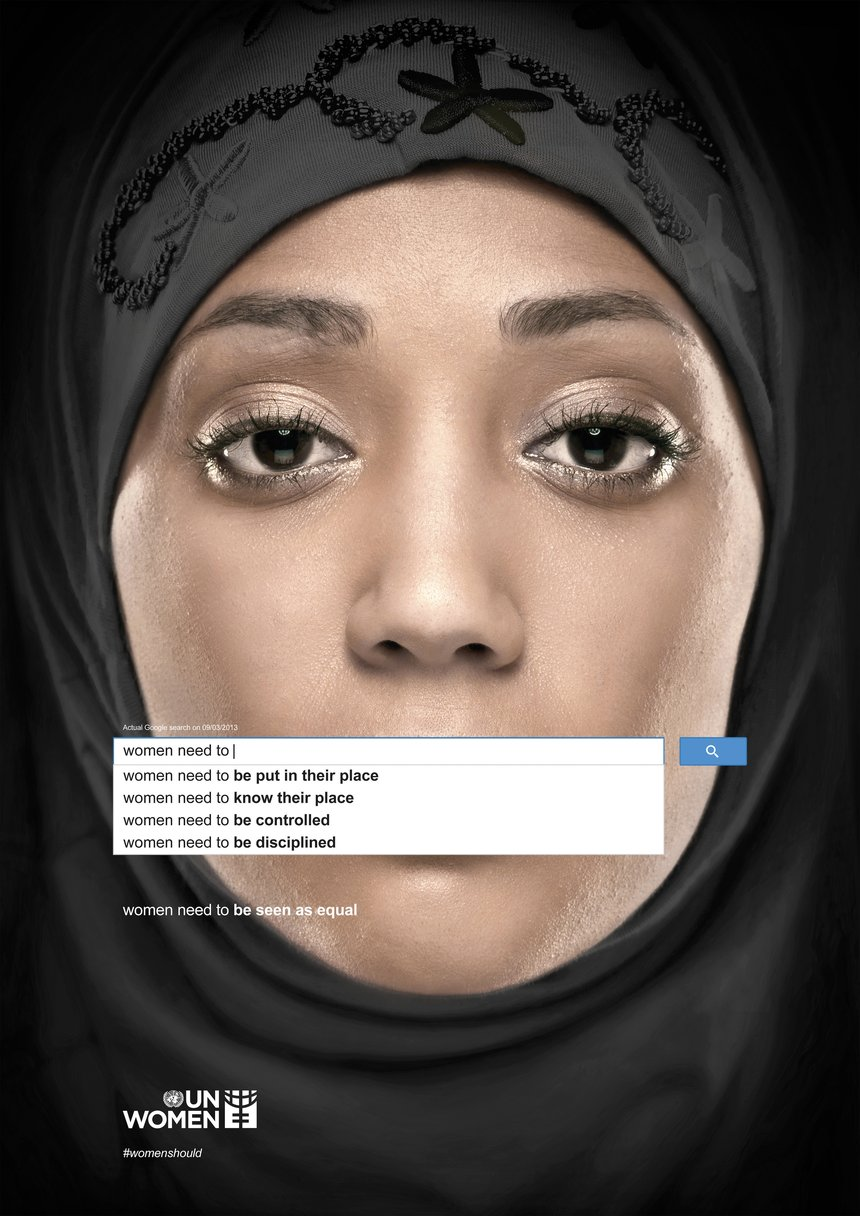
\includegraphics[width=150px]{campagne.jpg}
 \end{center}
 \caption{Extrait de la campagne \textit{The Autocomplete Truth} de l'ONU.}
 \label{campagne}
\end{figure}

L'autrice revient ensuite sur ses recherches à propos des algorithmes d'autocomplétion de Google, à travers un article qu'elle a co-signé avec Frédéric \textsc{Kaplan}, chaire de \textit{Digital Humanities} et directeur du laboratoire DHLab à Lausanne. Elle y explique notamment pourquoi ce mécanisme d'autocomplétion est une prothèse linguistique, c'est à dire qu'il est un relai entre la pensée et son expression écrite. Par sa suggestion a posteriori (l'autocomplétion intervient avant que l'utilisateur-ice ait terminé de saisir sa requête), l'autocomplétion peut accidentellement induire des recherches qu'une personne n'aurait pas cherché à la base et, dans le contexte qui nous intéresse, se faire le relai de stéréotypes négatifs. Ainsi, par effet de cercle vicieux, la présence de ces suggestions renforce les mécanismes d'oppressions, et ces mécanismes d'oppression augmentent les occurrences de ces suggestions stéréotypées. Ce mécanisme d'auto-renforcement est aussi à la base du concept de bulle de filtres, que l'on observe notamment sur Facebook \footnote{Jeff \textsc{Yates} a testé concrètement cet effet. \url{http://ici.radio-canada.ca/nouvelle/1029916/experience-facebook-algorithmes-bulle-desinformation?fromBeta=true}}, et qui peut induire un biais de confirmation énorme. Dans un autre registre, cet effet de cercle a pu s'observer quand \textit{Tay}, une intelligence artificielle conversationnelle mise sur Twitter à disposition du public par Microsoft, est devenu vulgaire et antisémite sous l'influence des conversations avec des trolls de l'\textit{alt-right}\footnote{\url{http://www.telegraph.co.uk/technology/2016/03/24/microsofts-teen-girl-ai-turns-into-a-hitler-loving-sex-robot-wit/}}.

Il serait cependant précipité d'attribuer à Google l'entière responsabilité de ces dérives. L'autrice suggère notamment le rôle des activistes méninistes et virilistes, qui opèrent un retour en force ces dernières années grâce à Internet et les réseaux sociaux. Cette mouvance souvent proche de l'extrême-droite se développe en réaction à une supposée ``crise de la masculinité'', et prône un retour à des valeurs patriarcales traditionnelles plaçant un sexe masculin fort comme pilier de la société. 

On voit bien ici que, comme vu plus haut, l'algorithme n'est absolument pas objectif, et qu'il est le produits de reflets multiples entre la mentalité de ces créateur-ice-s, et des individus qui se l'approprient dans son usage.

\subsection{Assurances et profilage}

Sous l'angle de la gouvernementalité algorithmique, on peut se poser la question des discriminations anticipatives dans les compagnie d'assurance sur la base des profils de risques. À partir du moment où on peut affiner ces risques, on ne peut plus concevoir l'assurance sociale qui d'après certains serait fondée sur une sorte de ``voile d'ignorance'' (John Rawls) ; c'est-à-dire que l'on n'accepterait de s'assurer mutuellement que parce qu'on ne connaît pas d'avance qui est porteur de quels types de risques. Si ce voile d'ignorance disparait, à savoir que l'on peut profiler les individus et leurs risques associés, le principe de solidarité à la base des systèmes d'assurance et de mutuelle s'évanouit : ``Pourquoi payer pour celleux qui ont plus de chances d'avoir des accidents que moi ?'' En retour, les prix sont aussi augmentés pour celles et ceux à facteur de risque plus élevé, ce qui introduit une discrimination supplémentaire.

\subsection{Vidéosurveillance, panoptique et sécuritarisme}

Dans \cite{nps}, Antoinette \textsc{Rouvroy} parle de l'émergence de la gouvernementalité algorithmique dans le domaine des connaissances des intentions criminelles, du souci de remplacer par des dispositifs technologiques moins onéreux le personnel de sécurité déployé dans tous les lieux stratégiques. C'est le principe du panoptique, avec par exemple INDECT, le projet européen de surveillance intelligente. Ce projet prévoit tout simplement une surveillance généralisée et intelligente (algorithmique) en milieu urbain via l'utilisation de caméras de surveillance, la géolocalisation des téléphones portables, la détection de ``données biométriques'' et la surveillance des données et fichiers échangés sur internet (un \textit{Big Brother}\footnote{En référence au roman d'anticipation dystopique de George \textsc{Orwell}.} européen).

Ce projet a bien évidemment été beaucoup critiqué.. La chercheuse Rosamunde \textsc{Van Brakel} du LSTS (\textit{Law, Science, Technology \& Society}) de l'ULB (Université Libre de Bruxelles) pense que le projet INDECT et les autres projets du même genre risquent non seulement, de par la marge d'erreur importante, d'accuser à tort certains individus, mais aussi de mener à une ``culture de la peur'' dans une société où ne règnerait plus la présomption d'innocence, mais la ``méfiance généralisée''. Selon elle, les ``indicateurs de méfiance'' utilisés pour détecter un suspect pourrait créer une forme de discrimination algorithmique. 

Cela soulève des questions de transparence et de responsabilité ; en effet, si les gens ne sont pas conscients de l'existence de cette technologie, comment sauront-ils que leurs droits (droit à la vie privée) ont été violés ? À contrario, si les gens sont au courant de l'existence de ce type de technologie, ils pourraient modifier leurs comportements et traiter les personnes qui se comportent ``anormalement'' avec peur et méfiance. Cela peut conduire à un tri social, et là encore à une discrimination. 

La façon dont le logiciel est conçu peut avoir un impact sur qui est considéré comme suspect et qui ne l'est pas. Certains indicateurs de la suspicion pourraient être fondés sur des hypothèses erronées et sur des préjugés indirects. Comment distinguer quelqu'un qui envisage le suicide, quelqu'un qui est juste très nerveux (par exemple qui a un entretien d'embauche), quelqu'un avec un trouble psychiatrique et un ``terroriste potentiel'' ? ``L'anneau d'acier'' Londonien, qui comprend rien moins qu'un demi million de caméras, a permis d'arrêter en moins d'une semaine les terroristes (et leurs complices) qui tentèrent d'attaquer le métro et le bus en juillet 2005. Néanmoins, les policiers abattirent également Jean Charles \textsc{de Menezes} soupçonné par erreur.

\section{Reprendre le contrôle des systèmes de prise de décision pour une gouvernementalité citoyenne}

Nous venons de soulever bon nombre de problèmes liées à l'utilisation d'algorithmes dans la chaîne décisionnelle. Afin d'éviter de noircir plus que de mesure le tableau, on peut relever un certain nombres de solutions pour lutter contre ces biais. La loi d'abord, peut encadrer les politiques de collecte et d'analyse des données, afin de prévenir certaines dérives liées au profilage. Mais nous allons voir qu'une autre solution est possible.

Bernard Stiegler, philosophe et directeur de l'institut de recherche et d'innovation, enseignant à l'UTC, interviewé dans le cadre d'un épisode de l'émission \#DATAGUEULE sur les mutations du travail\footnote{\url{https://www.youtube.com/watch?v=4n2tWyIuA8g}}, dénonce la prolétarisation du travail, c'est à dire la perte de sens dans un système ultra-taylorisé\footnote{Le taylorisme est une doctrine de rationnalisation du travail. C'est, avec entres-autres le fordisme, l'une des méthodes d'Organisation Scientifique du Travail.}, ultra-rationnalisé, et  de plus en plus opaque pour les individus. Dans la société néolibérale, rationnalisée à l'extrême, les employé-e-s en viennent à être remplacés par des machines commandées par des algorithmes, comme nous l'avons vu tout au long de ce rapport. Selon Bernard Stiegler, les employé-e-s sont porteur/euses d'une composante qui ne peut être automatisée, et qui est vecteure de différenciation. Cette perte d'emploi que créent les algorithmes, il essaye de la voir comme une chance de modifier notre rapport au travail et à l'économie, sous une approche plus solidaire, qui permet de créer du savoir collectif. L'outil numérique peut jouer un rôle essentiel dans ces mutations. Mal utilisé, il a certes engendré Uber, Google, qui avec leurs algorithmes de profilage captent la valeur et fragilisent la société, et bien sûr créent tous les problèmes de discrimination algorithmique précédemment évoqués. Mais mieux utilisé, le numérique peut aussi servir à recréer du lien entre les individus : le tout est de ne plus déléguer les prises de décision à des algorithmes, mais à des réunions publiques, dans lesquelles les acteurs et actrices de la vie en société ne sont plus les grosses entreprises par le biais des algorithmes, mais le peuple dans son ensemble. Dans ce cadre là, l'analyse de données fournit alors des indicateurs pour informer les individus et leur permettre de prendre des décisions, augmentant ainsi l'intelligence collective : c'est ce qu'Émile Durkheim appelait la solidarité organique, à l'inverse de la société actuelle, fragmentée et individualisée par l'économie spéculative et le capitalisme.

On peut trouver un exemple très concret d'application de cette théorie dans Mastodon, réseau social libre et décentralisé sur lequel nous allons nous attarder un moment avant de conclure ce rapport. Mastodon est une implémentation de OStatus, un standard pour le microblogging fédéré. En effet, à l'instar de Twitter, Mastodon permet de partager des messages courts (500 caractères contre 140 pour Twitter), enrichis parfois d'images, de liens, et avec lesquels les autres utilisateur/ices peuvent interragir (les mettre en favori, les repartager sur leur propre fil, y répondre, etc.). Mais là où Mastodon se distingue de Twitter, c'est qu'au lieu d'être un service centralisé et distribué par une entreprise, chacun-e peut déployer sa propre instance de Mastodon sur sa propre infrastructure, instance qui se fédère au reste du ``fediverse'' OStatus\footnote{Il s'agit des autres instances Mastodon, mais aussi des instances GNU social, une autre implémentation de OStatus plus ancienne.}. Les administrateur/ices de chaque instance peuvent alors proposer leur propre politique de modération, en réponse à Twitter qui a été ces derniers temps pointé du doigt pour sa politique de modération à double vitesse\footnote{Twitter, comme Facebook, a une grande tolérance pour les propos sexistes, racistes, néonazis ou appelant au harcèlement. De nombreuses personnalités féministes sur Twitter ont dénoncé l'impunité des trolls d'extrême droite de 4chan aux US, ou du blabla 18-25 de jeuxvideo.com, qui menacent et orchestrent régulièrement le harcèlement de la communauté féministe et queer sur Internet.}. On a ainsi observé l'apparition en France de nombreuses instances qui se posent en \textit{safe spaces} pour permettre aux personnes oppressées (LGBTQI+ notamment) de s'exprimer sans craindre le harcèlement (figure \ref{masto-love}).

\begin{figure}[ht]
 \begin{center}
  
\includegraphics[width=180px]{witches.png}
  
\includegraphics[width=180px]{octodon.png}
  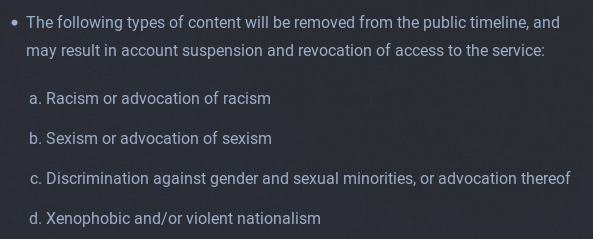
\includegraphics[width=180px]{mastodon.png}
 \end{center}
 \caption{Extraits des politiques de modération de quelques instances Mastodon (de gauche à droite et de haut en bas : witches.town, octodon.social, mastodon.social).}
 \label{masto-love}
\end{figure}

Il est à noter d'ailleurs que Mastodon a été créé par Eugen \textsc{Rochko}, militant queer allemand, et qu'à ce titre Mastodon inclut un certain nombre de fonctionnalités allant dans ce sens : système de \textit{Content Warning}\footnote{Le système de \textit{Content Warning} dissimule le texte du post, le remplaçant par un avertissement de contenu personnalisable qui permet à tout à chacun-e de choisir ou non de révéler le texte, selon sa sensibilité personnelle} intégré, plateforme d'administration permettant simplement de bloquer des instances qui auraient un discours nuisible\footnote{Notamment, nombre d'instances GNU Social, comme ``unsafe.space'' (le nom en dit long), existent en réaction à une soit disante atteinte à la liberté d'expression de la part des ``\textit{Social Justice Warriors}''. À ce propos, il est bon de partager cette planche de xkcd sur le sujet : \url{https://xkcd.com/1357/}.}

On a pu ainsi voir concrètement avec Mastodon comment la décentralisation des données peut être un moyen de se mettre à l'abri de l'ingérence des géants du web, maîtres de la collecte de données : non seulement en reprenant le contrôle de ses données personnelles, mais aussi par la création d'espaces communautaires de taille plus réduite ou le lien social est plus étroit. On constate souvent que les membres des instances de taille petite à moyenne connaissent au moins de vue les administrateur/ices et modérateur/ices, et qu'un lien de confiance se tisse. Un moyen concret de lutter contre les discriminations algorithmiques, en plus d'arrêter de déléguer la prise de décision aux algorithmes, passe alors aussi par une redécentralisation d'Internet pour un meilleur contrôle de ses données personnelles.

\chapter*{Conclusion}
\addcontentsline{toc}{chapter}{Conclusion}

Nous avons brièvement vu dans ce rapport que l'on peut effectivement dire qu'il existe une discrimination algorithmique. Les algorithmes, par leur omnipotence, confèrent à ceux qui les contrôlent un pouvoir économique et politique majeur qui peut être nuisible à la société s'il n'est pas régulé. Leurs limites et leurs incapacités à se poser en analystes neutres et objectifs du monde illustrent la nécessité de cette régulation, pour établir une gouvernementalité qui ne serait pas fondée sur les seules valeurs qu'essayent d'imposer les grandes entreprises. Bien sûr, des solutions existent, et nous n'avons fait qu'en effleurer la surface. Mais la (relative) popularité du logiciel libre, porteur d'une éthique respectueuse des libertés fondamentales, illustre le désir des citoyen-ne-s d'être acteur/ices du monde, et pas simplement consommateur/ices. \textit{La route est longue, mais la voie est libre}\footnote{Slogan de Framasoft, association française militant pour sensibiliser la société aux valeurs portées par le logiciel libre.}, comme disait l'autre !

\begin{quotation}
 Face à la rapidité de calcul des algorithmes, il n’est rien de plus confondant que la lenteur des parlements et des juges. Car s’il faut réguler les algorithmes, il faudra agir rapidement et avec détermination (Étienne Papin, avocat, \textit{in} \underline{Si les algorithmes nous régulent faut-il réguler les algorithmes ?})
\end{quotation}


\appendix
\bibliographystyle{alpha}
\bibliography{rapport}
\addcontentsline{toc}{chapter}{Bibliographie supplémentaire}

\end{document}